\documentclass[12pt]{article}

\title{ET4340 Electronics for Quantum Computing\\Homework 4}
\author{
    Mick van Gelderen\\4091566
}
\date{November 2013}

\usepackage[utf8]{inputenc}
\usepackage[a4paper,margin=2.2cm]{geometry}
\usepackage{natbib}
\usepackage{graphicx}
\usepackage{listings}
\usepackage{framed}
\usepackage{mathtools}
\usepackage{braket}
\usepackage{ifmtarg}
\usepackage{multirow}
\usepackage{xfrac}

\newcommand{\pauli}[1]{
    \ensuremath{
        \begin{pmatrix}
            \if#1x
                0 & 1 \\
                1 & 0 \\
            \fi\if#1y
                0 & -i \\
                i & 0 \\
            \fi\if#1z
                1 & 0 \\
                0 & -1 \\
            \fi
        \end{pmatrix}
    }
}

\setlength{\parindent}{0cm}

\newcommand{\paulisigma}[1]{%
    \ensuremath{\sigma{}_{#1}}%
}

\newcommand{\pmat}[1]{\begin{pmatrix}#1\end{pmatrix}}
\newcommand{\rsqrt}[1]{\ensuremath{\frac{1}{\sqrt{#1}}}}

\setlength{\parskip}{0.5em plus4mm minus3mm}
\newenvironment{answer}{\begingroup\setlength{\leftskip}{-\leftmargin}\begin{framed}}{\end{framed}\endgroup}

\newcommand{\CNOT}[1]{\ensuremath{\texttt{CNOT}_{#1}}}
\newcommand{\CPHASE}[1]{\ensuremath{\texttt{CPHASE}_{#1}}}
\newcommand{\SWAP}[1]{\ensuremath{\texttt{SWAP}_{#1}}}
\newcommand{\cnotgr}[1]{\ensuremath{\pmat{%
        1 & 0 & 0 & 0 \\%
        0 & 1 & 0 & 0 \\%
        0 & 0 & 0 & 1 \\%
        0 & 0 & 1 & 0 \\%
}}}

\begin{document}

\maketitle
\hfill\\\\\\

\paragraph{Problem 1: Quantum Fourier Transform} \hfill \\

\begin{enumerate}

    \item Write the $8\times8$ matrix (in the computational basis) corresponding to the quantum Fourier transform on a 3-qubit register.

    \begin{answer}
        The matrix $U_{QFT,8}$ is defined as:
        \begin{align*}
            U_{QFT,8} = \rsqrt{N}\sum\limits_{l = 0}^{N - 1}\sum\limits_{k = 0}^{N - 1}e^{\frac{i2\pi{}lk}{N}}\ket{l}\bra{k}
        \end{align*}
        where $N = 8$.
        \begin{align*}\pmat{
            1 &  1 &  1 &  1 &  1 &  1 &  1 &  1 \\
            1 &  \sqrt{2} + \sqrt{2}i & i & -\sqrt{2} + \sqrt{2}i & -1 & -\sqrt{2} - \sqrt{2}i & -i &  \sqrt{2} - \sqrt{2}i \\
            1 & i & -1 & -i &  1 & i & -1 & -i \\
            1 & -\sqrt{2} + \sqrt{2}i & -i &  \sqrt{2} + \sqrt{2}i & -1 &  \sqrt{2} - \sqrt{2}i & i & -\sqrt{2} - \sqrt{2}i \\
            1 & -1 &  1 & -1 &  1 & -1 &  1 & -1 \\
            1 & -\sqrt{2} - \sqrt{2}i & i &  \sqrt{2} - \sqrt{2}i & -1 &  \sqrt{2} + \sqrt{2}i & -i & -\sqrt{2} + \sqrt{2}i \\
            1 & -i & -1 & i &  1 & -i & -1 & i \\
            1 &  \sqrt{2} - \sqrt{2}i & -i & -\sqrt{2} - \sqrt{2}i & -1 & -\sqrt{2} + \sqrt{2}i & i &  \sqrt{2} + \sqrt{2}i \\
        }\end{align*}
    \end{answer}

    \item Show that this matrix is unitary

    \begin{answer}
        Use a computer to calculate $U_{QFT}U_{QFT} = I$. You can easily see that the matrix is symmetric so this is the only thing we have to show.
        Matlab indeed gives $I$ with some near zero imaginary parts.
    \end{answer}

    \item Draw the quantum circuit that implements this QFT

    \begin{answer}
        From the lecture slides where it was drawn for 4 qubits:
        \begin{center}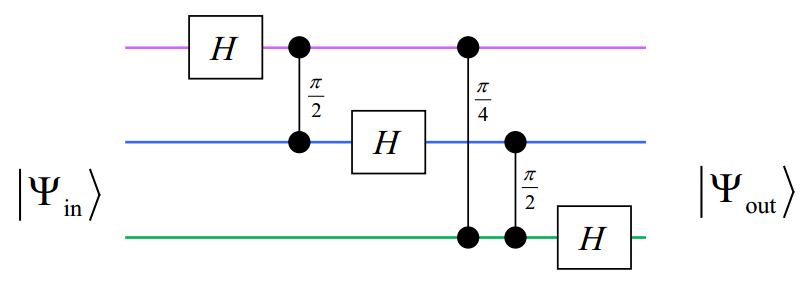
\includegraphics[width=.8\textwidth]{problem-1.png}\end{center}
    \end{answer}

\end{enumerate}

\paragraph{Problem 2: Generalized quantum kick-back} \hfill \\

In the lectures, we have seen how the Deutsch and Bernstein-Vazirani quantum games exploit quantum kick-back to efficiently extract properties of $n$-to-1 bit boolean functions. In this problem, we generalize quantum kick-back to $n$-to-$m$ bit boolean functions encoded in unitary functions as usual: $U_f\ket{x}\ket{y} = \ket{x}\ket{(y + f(x)) \mod M}$ for computational states $\ket{x}$ and $\ket{y}$ in the top and bottom registers, respectively. Consider the circuit below.

\begin{center}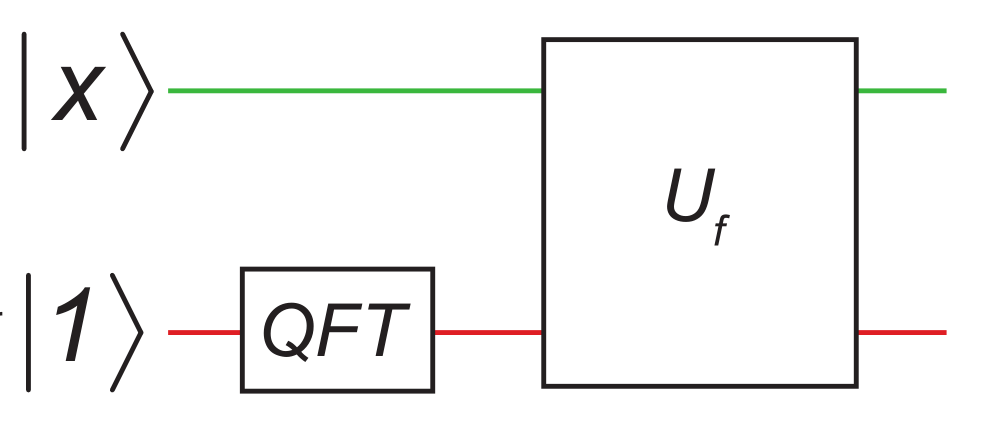
\includegraphics[width=.5\textwidth]{problem-2.png}\end{center}

\begin{enumerate}

    \item What is the state of the bottom register after application of the m-bit QFT on the initial
state $\ket{1} = \ket{00000...1}$?

    \begin{answer}
        $U_{QFT}\ket{1}$ equals the last column of $U_{QFT}$. So $U_{QFT}\ket{1} = \rsqrt{N}\sum\limits_{k = 0}^{N - 1}e^{\frac{i2\pi{}(N - 1)k}{N}}\ket{k}$
    \end{answer}

    \item Now apply $U_f$, with the top register starting in a computational state $\ket{x}$. What is the combined state of the top and bottom registers immediately after $U_f$? Show that this this state can be rewritten as:

    \begin{align*}
        e^{\frac{-i2\pi{}f(x)}{M}}\ket{x}\otimes{}U_{QFT}\ket{1},
    \end{align*}

    where $M = 2^m$. Evidently, the top and bottom registeres are not entangled, and $f(x)$ is encoded in the quantum phase of the probability amplitude!

    \begin{answer}
        ?
    \end{answer}

    \item Finally, consider the case that the top register is initialized in the maximal superposition state $\rsqrt{N}(\ket{0} + \dots + \ket{N - 1})$. As usual, $N = 2^n$. What will be the final state after application of $U_f$?

    \begin{answer}
        ?
    \end{answer}

\end{enumerate}

\paragraph{Problem 3: Breaking RSA}

In this exercise, we will break RSA by period finding. $N$ will be small enough that we will find periods by brute force.

\begin{enumerate}
    \item List the integers $a < N$ that are co-prime with $N$. Let us pick one of these integers: let us agree to all `randomly' pick $a = 8$.

    \begin{answer}
        I guess $N = 21$.
        \begin{tabular}{c|l|l}
            $n$ & divisible by & co-primes\\
            \hline
            2 & 2 & 1 \\
            3 & 3 & 1 2 \\
            4 & 2 4 & 1 3 \\
            5 & 5 & 1 2 3 4 \\
            6 & 2 3 6 & 1 5 \\
            7 & 7 & 1 2 3 4 5 6 \\
            8 & 2 4 8 & 1 3 5 7 \\
            9 & 3 9 & 1 2 4 5 7 8 \\
            10 & 2 5 10 & 1 3 7 9 \\
            11 & 11 & 1 2 3 4 5 6 7 8 9 10 \\
            12 & 2 3 4 6 12 & 1 5 7 11 \\
            13 & 13 & 1 2 3 4 5 6 7 8 9 10 11 12 \\
            14 & 2 7 14 & 1 3 5 6 9 11 13 \\
            15 & 3 5 15 & 1 2 4 7 8 11 13 14 \\
            16 & 2 4 8 16 & 1 3 5 7 9 11 13 15 \\
            17 & 17 & 1 2 3 4 5 6 7 8 9 10 11 12 13 14 15 16 17 \\
            18 & 2 3 6 9 18 & 1 5 7 11 13 17 \\
            19 & 19 & 1 3 5 7 8 9 10 11 12 13 14 15 16 17 18 19 \\
            20 & 2 4 5 10 20 & 1 3 7 9 11 13 17 19 \\
            21 & 3 7 21 & 1 2 4 5 8 10 11 13 16 17 19 \\
        \end{tabular}
    \end{answer}

    \item Compute $8^0 \mod 21$, $8^1 \mod 21$, \ldots until you discover the period $r$ of $f(x) = 8^x \mod 21$.

    \begin{answer}
        \begin{tabular}{c|c}
            $n$ & $8^n \mod 21$ \\
            \hline
            0 & 1 \\
            1 & 8 \\
            2 & 1 \\
        \end{tabular}
        The period seems to be $2$.
    \end{answer}

    \item Find the greatest common denominator (gcd) between, $8^{\sfrac{r}{2}} + 1$ and $21$. Check whether the result is a prime factor of 21.

    \begin{answer}
        Since $r = 2$, $8^{\sfrac{r}{2}} + 1 = 9$. The gcd of $9$ and $21$ is $3$ which is indeed a prime factor of $21$.
    \end{answer}

    \item Similarly, find the gcd between $8^{\sfrac{r}{2}} - 1$ and $21$.

    \begin{answer}
        The gcd of $7$ and $21$ is $7$ which is a prime factor of $21$.
    \end{answer}

    \item Repeat the process for $a = 10$.

    \begin{answer}
        Finding the period:
        \begin{tabular}{c|c}
            $n$ & $10^n \mod 21$ \\
            \hline
            0 & 1 \\
            1 & 10 \\
            2 & 6 \\
            3 & 13 \\
            4 & 4 \\
            5 & 19 \\
            6 & 1 \\
        \end{tabular}
        The period seems to be $6$.
        The gcd's of $10^3 \pm 1$ and $21$ are $3$ and $7$, magic!
    \end{answer}
\end{enumerate}

\paragraph{Problem 4: Breaking RSA with Shor's algorithm} \hfill \\

Now we will go through the steps of Shor's algorithm in order to find the period $r$ of $8^x\mod21$. For simplicity, lest us use just four qubits for the top register which is enough for our choice of $a = 8$.
\emph{Note: Please use decimal bra-ket notation instead of binary. }

\begin{enumerate}
    \item Initialize each register to $\ket{0}$.
\end{enumerate}


\end{document}

